%! Author = vladislav.yaroshchuk
%! Date = 10/10/2021

\pagebreak


\section{Определение номенклатуры документов.}

Шаблоном процессов сопровождения и их документирования был выбран проект QEMU\cite{qemu,qemucontribute}.
Ниже представлена упрощенная диаграмма процесса сопровождения.

\begin{figure}[ht]
    \begin{center}
        \scalebox{0.4}{
            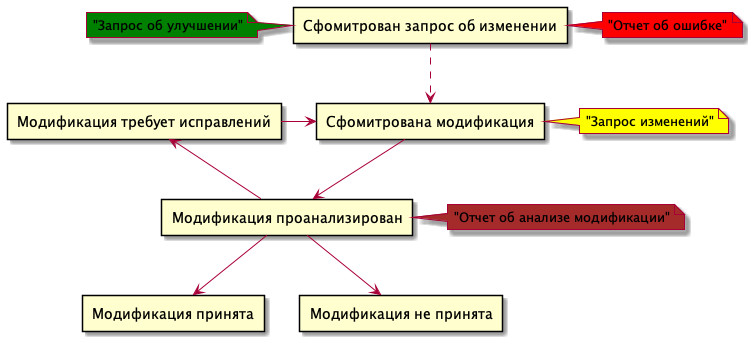
\includegraphics{images/maintenance_process}
        }
    \end {center}\label{fig:maintenance_process}
\end {figure}

Таким образом, получаем список документов:

\begin{itemize}
    \item План сопровождения -- описывает методы сопровождения, необходимые ресурсы и работы применительно к сопровождению.

    \item Отчет о проблеме -- описывает обнаруженную в продукте проблему

    \item Запрос об улучшении -- описывает требования к улучшению продукта, но не конкретные изменения

    \item Описание модификации -- описывает изменения в продукте, предполагаемые к включению в следующей версии продукта

    \item Отчет об анализе модификации -- описывает мнение отвественного (авторитетного) лица касательно Модификации

    \item Отчет об изменениях в версии -- описывает изменения в продукте в сравнении с предыдущей версией
\end{itemize}
